% Ejemplo de documento LaTeX
% Tipo de documento y tamaño de letra
\documentclass[10pt]{article}
% Preparando para documento en Español.
% Para documento en Inglés no hay que hacer esto.
\usepackage[spanish]{babel}
\selectlanguage{spanish}
\usepackage[utf8]{inputenc}


% EL titulo, autor y fecha del documento
\title{Tiro parabólico con FORTRAN y gnuplot}
\author{Rios Quijada Danira}
\date{10 de Marzo de 2015}
% Aqui comienza el cuerpo del documento
\usepackage{graphicx}
\begin{document}
% Construye el título
\maketitle
\section{Tiro parabólico con FORTRAN}
En esta práctica, primeramente realizamos un programa en FORTRAN para calcular la posición de un objeto lazado con tiro parabólico, en ciertos instantes de tiempo, el programa también calcula la y máxima y la x máxima,asi como el tiempo total en el aire; todo esto dependiendo de la velocidad inicial y del ángulo de tiro.Todos estos calculos se basan en las ecuaciones de tiro parabólico, descritas a continuación:
\space
\space  
\begin{tabular}{l}
$x=v_{0}tcos(\theta)$\\
$y=v_{0}tsin(\theta)- \frac{1}{2}gt^2$

\end{tabular}

\subsection{Código}
\begin{tabular}{l}
El código que utilizamos para realizar el programa fue el siguiente:\\

\begin{verbatim}  
 !************************************************  
  !This program plots projectile motion of an object.  
  !The program requires user input for initial velocity   
  !and angle of the object.The algorithm uses a time   
  !step of 0.01 second i.e. it calculates object's  
  !location in the x and y plane every 0.01 second.  
  !**********By: Waleed Ishaque, 2013**************  
  program tiro_parabolico  
       implicit none  
       !Defining constants:  
      real, parameter :: pi = 4.0*atan(1.0) 
       real :: v, a, t, r, vx, vy, xm, ym  
       real, parameter :: g = 9.81  
      real:: x(150),y(150)  

          integer :: i 


      !donde g es la aceleracion de la gravedad, pi is "pi"   

      !v es la velocidad inicial del objeto   

       !a es el angulo de tiro, r es el mismo angulo, pero en radianes   

      !t es el tiempo   

      !x and y son cordenadas del objeto durante el tiro    

      !Seek user input   

       write(*,*) 'Dame el ángulo inicial de tiro del proyectil en grados (Real)'   

      read *, a   

       write(*,*) 'Dame la velocidad inicial del proyectil en m/s (Real) '   

       read *, v   

       !Convirtiendo los grados  a radianes   

       r = a*pi/180.0  

       ! Calculando las velocidades en los 2 ejes

       vx=(v)*(cos(r))

       vy=(v)*(sin(r))

       !open .dat file and start writing on it using the algorithm   

       open(1, file='tiro.dat')   

        x=0
        y=0 

       do i=1,100   

            !displacement of object in x and y direction   

           t = (float(i)*0.01)   

            x(i) = vx*t   

            y(i) = (vy*t) - (0.5*g*t*t)   

           !write output in file "proj.dat" for plotting   

            write(1,*) x(i), y(i)   

           !kill the loop when the object hits the ground   

            if (y(i)<0) exit   

       end do   

      close(1)   

      !close file 
ym = (vy**2)/(19.6)
xm = x(i)
if (vx<0) then
xm = 0
end if
!resultados en pantalla
write(*,*) '^^^^^^^^^^^^^^^^^^^^^^^^^^^^^^^^^^^^^^^^^^^^^^^^^^^^^^^^^^^^^^^'
write(*,*) 'Un proyectil con una velocidad inicial de',v,'m/s'
write(*,*) 'y con un ángulo de tiro de',a, 'grados'
write(*,*)  'Alcanzará una h máxima de',ym, 'metros'
write(*,*) 'Su alcanze horizontal sera de',xm, 'metros'
write(*,*) 'y durará en el aire un tiempo de',t,'segundos'

  end program tiro_parabolico 

\end{verbatim} \\
\end{tabular}
\newpage
\subsection{Resultados}
Cabe denotar que en el código se cambia la salida estándar de los datos de posición a un archivo, llamado ``tiro.dat'', el cual utilizaremos posteriormente para graficar con gnuplot.una vez concluido el programa, lo compilamos, he aquí los resultados al ejecutarlo con los ángulos de 90,0, 60 y 30 grados.

\subsubsection{90 grados}
\begin{center}
   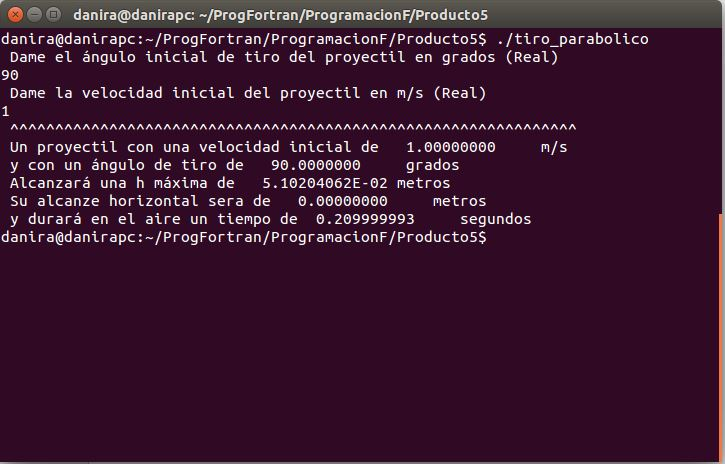
\includegraphics[scale=0.5]{tiro90.JPG}
\end{center}

\subsubsection{0 grados}
\begin{center}
   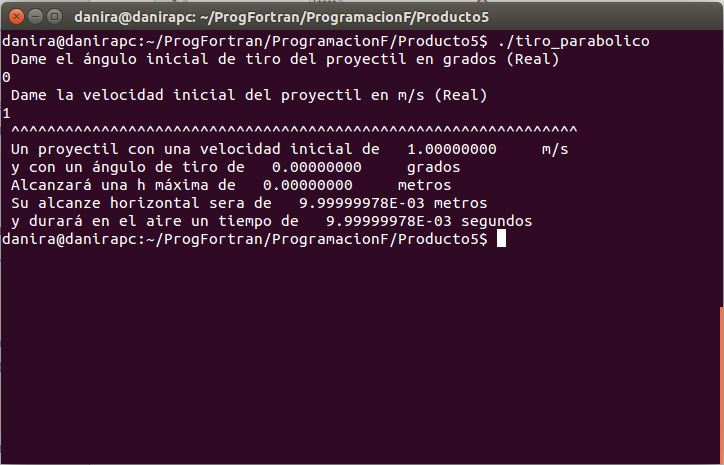
\includegraphics[scale=0.5]{tiro0.JPG}
\end{center}

\subsubsection{60 grados}
\begin{center}
   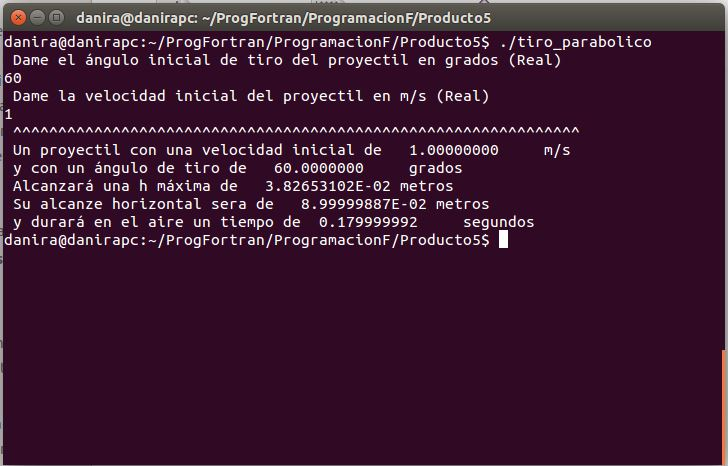
\includegraphics[scale=0.5]{tiro60.JPG}
\end{center}

\subsubsection{30 grados}
\begin{center}
   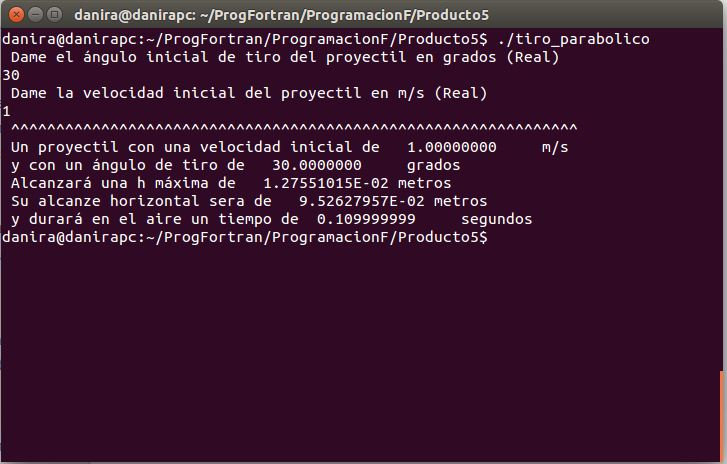
\includegraphics[scale=0.5]{tiro30.JPG}
\end{center}





\newpage


\section{Graficando con Gnuplot}
En esta parte de la práctica nos enfocamos en graficar la información que nos arrojó el archivo ``tiro.dat'', para eso utilizamos gnuplot y el siguiente código.


\begin{tabular}{l}
\begin{verbatim}  
 gnuplot>set term png
 gnuplot>set output 'tirogrados.png'
 gnupltot>plot 'tiro.dat'
\end{verbatim}\\
Obteniendo el siguiente resultado para cada ángulo de prueba;
\end{tabular}

\subsection{90 grados}
\begin{center}
   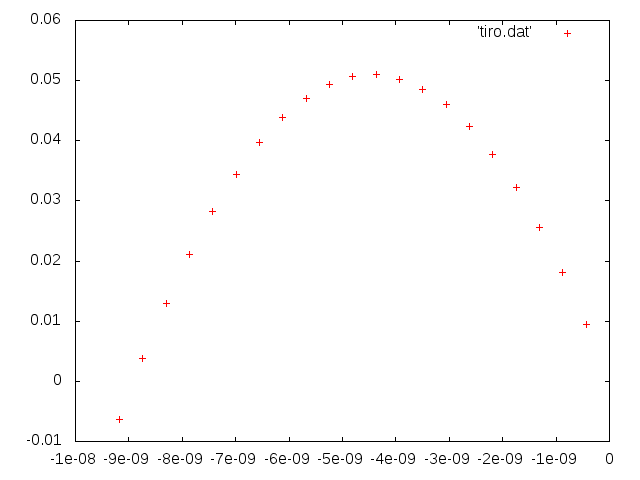
\includegraphics[scale=0.5]{tiro90.png}
\end{center}

\subsection{0 grados}
\begin{center}
   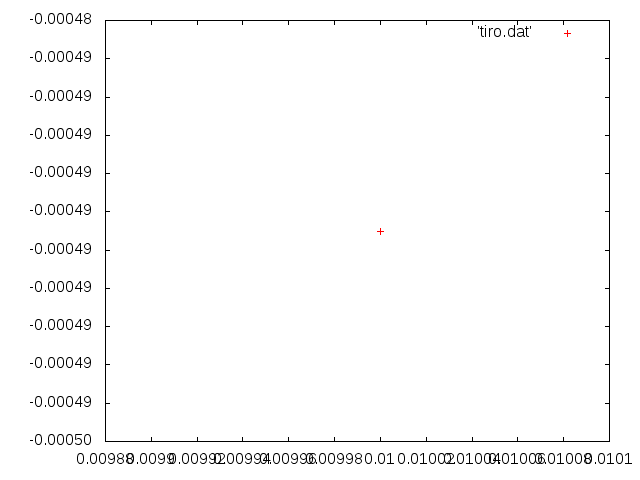
\includegraphics[scale=0.5]{tiro0.png}
\end{center}

\subsection{60 grados}
\begin{center}
   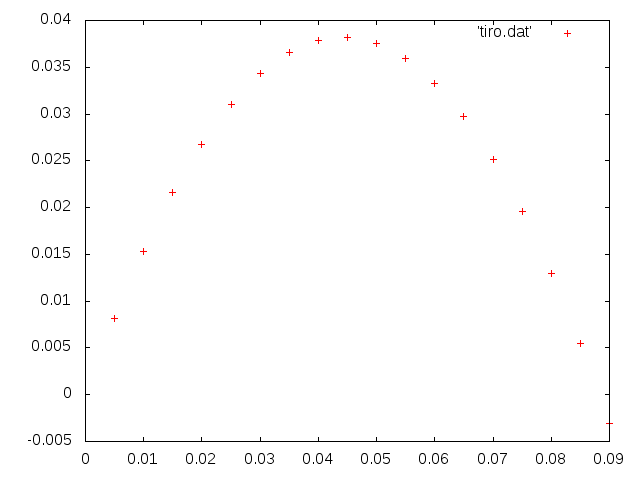
\includegraphics[scale=0.5]{tiro60.png}
\end{center}

\subsection{30 grados}
\begin{center}
   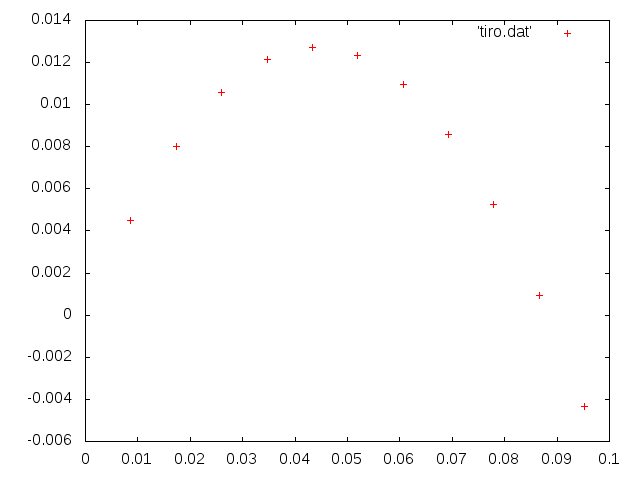
\includegraphics[scale=0.5]{tiro30.png}
\end{center}













% Nunca debe faltar esta última linea.
\end{document}
